
\subsubsection{5.1 RQ1: Trustworthiness Dimensions Are Significantly Correlated (H-E1)}

After controlling for model scale and RLHF status, \textbf{8 of 15} trustworthiness dimension pairs exhibit statistically significant partial Spearman correlations at the Bonferroni-corrected threshold.

\textbf{Table 1: All partial Spearman correlations, selected (n=16 models, Bonferroni-corrected $\alpha =0.0033)$}

\begin{table}[htbp]
\centering
\resizebox{\columnwidth}{!}{%
\begin{tabular}{llll}
\toprule
Pair & $\rho_{partial}$ & p-value & Significant \\
\midrule
Safety --- Privacy & **0.971** & 8.77e-09 & Yes \\
Fairness --- Privacy & 0.912 & 2.41e-06 & Yes \\
Privacy --- Machine\_Ethics & 0.859 & 1.64e-05 & Yes \\
Safety --- Machine\_Ethics & 0.841 & 3.22e-05 & Yes \\
Fairness --- Machine\_Ethics & 0.821 & 7.12e-05 & Yes \\
Truthfulness --- Fairness & 0.734 & 9.84e-04 & Yes \\
Truthfulness --- Safety & 0.698 & 2.31e-03 & Yes \\
Robustness --- Truthfulness & 0.612 & 1.17e-02 & No (borderline; does not pass Bonferroni) \\
Safety --- Robustness & $-0.188$ & 0.519 & No \\
\bottomrule
\end{tabular}
}
\end{table}

The 7 remaining pairs (not shown) also fall below the Bonferroni threshold.

Key observations:

\begin{enumerate}
\item \textbf{Safety--privacy is the strongest pair ($\rho$ = 0.971, p = 8.77e-9).} Privacy was originally predicted to be RLHF-insensitive; instead it shows stronger co-movement with safety than any other pair.
\end{enumerate}

\begin{enumerate}
\item \textbf{Robustness stands apart.} After full partial control ($\log_{10}(\text{params})$ + is\_RLHF), adversarial robustness has no Bonferroni-significant correlation with any other dimension. The safety--robustness partial correlation is directionally negative ($\rho = -0.188)$ but not significant.
\end{enumerate}

\begin{enumerate}
\item \textbf{Confound removal amplifies correlations for the RLHF-shaped cluster.} Raw Spearman for safety--privacy is $\rho_{raw}$ = 0.73, substantially below the partial $\rho$ = 0.971, illustrating that scale confound suppresses the estimate before removal.
\end{enumerate}

\begin{figure}[htbp]
\centering
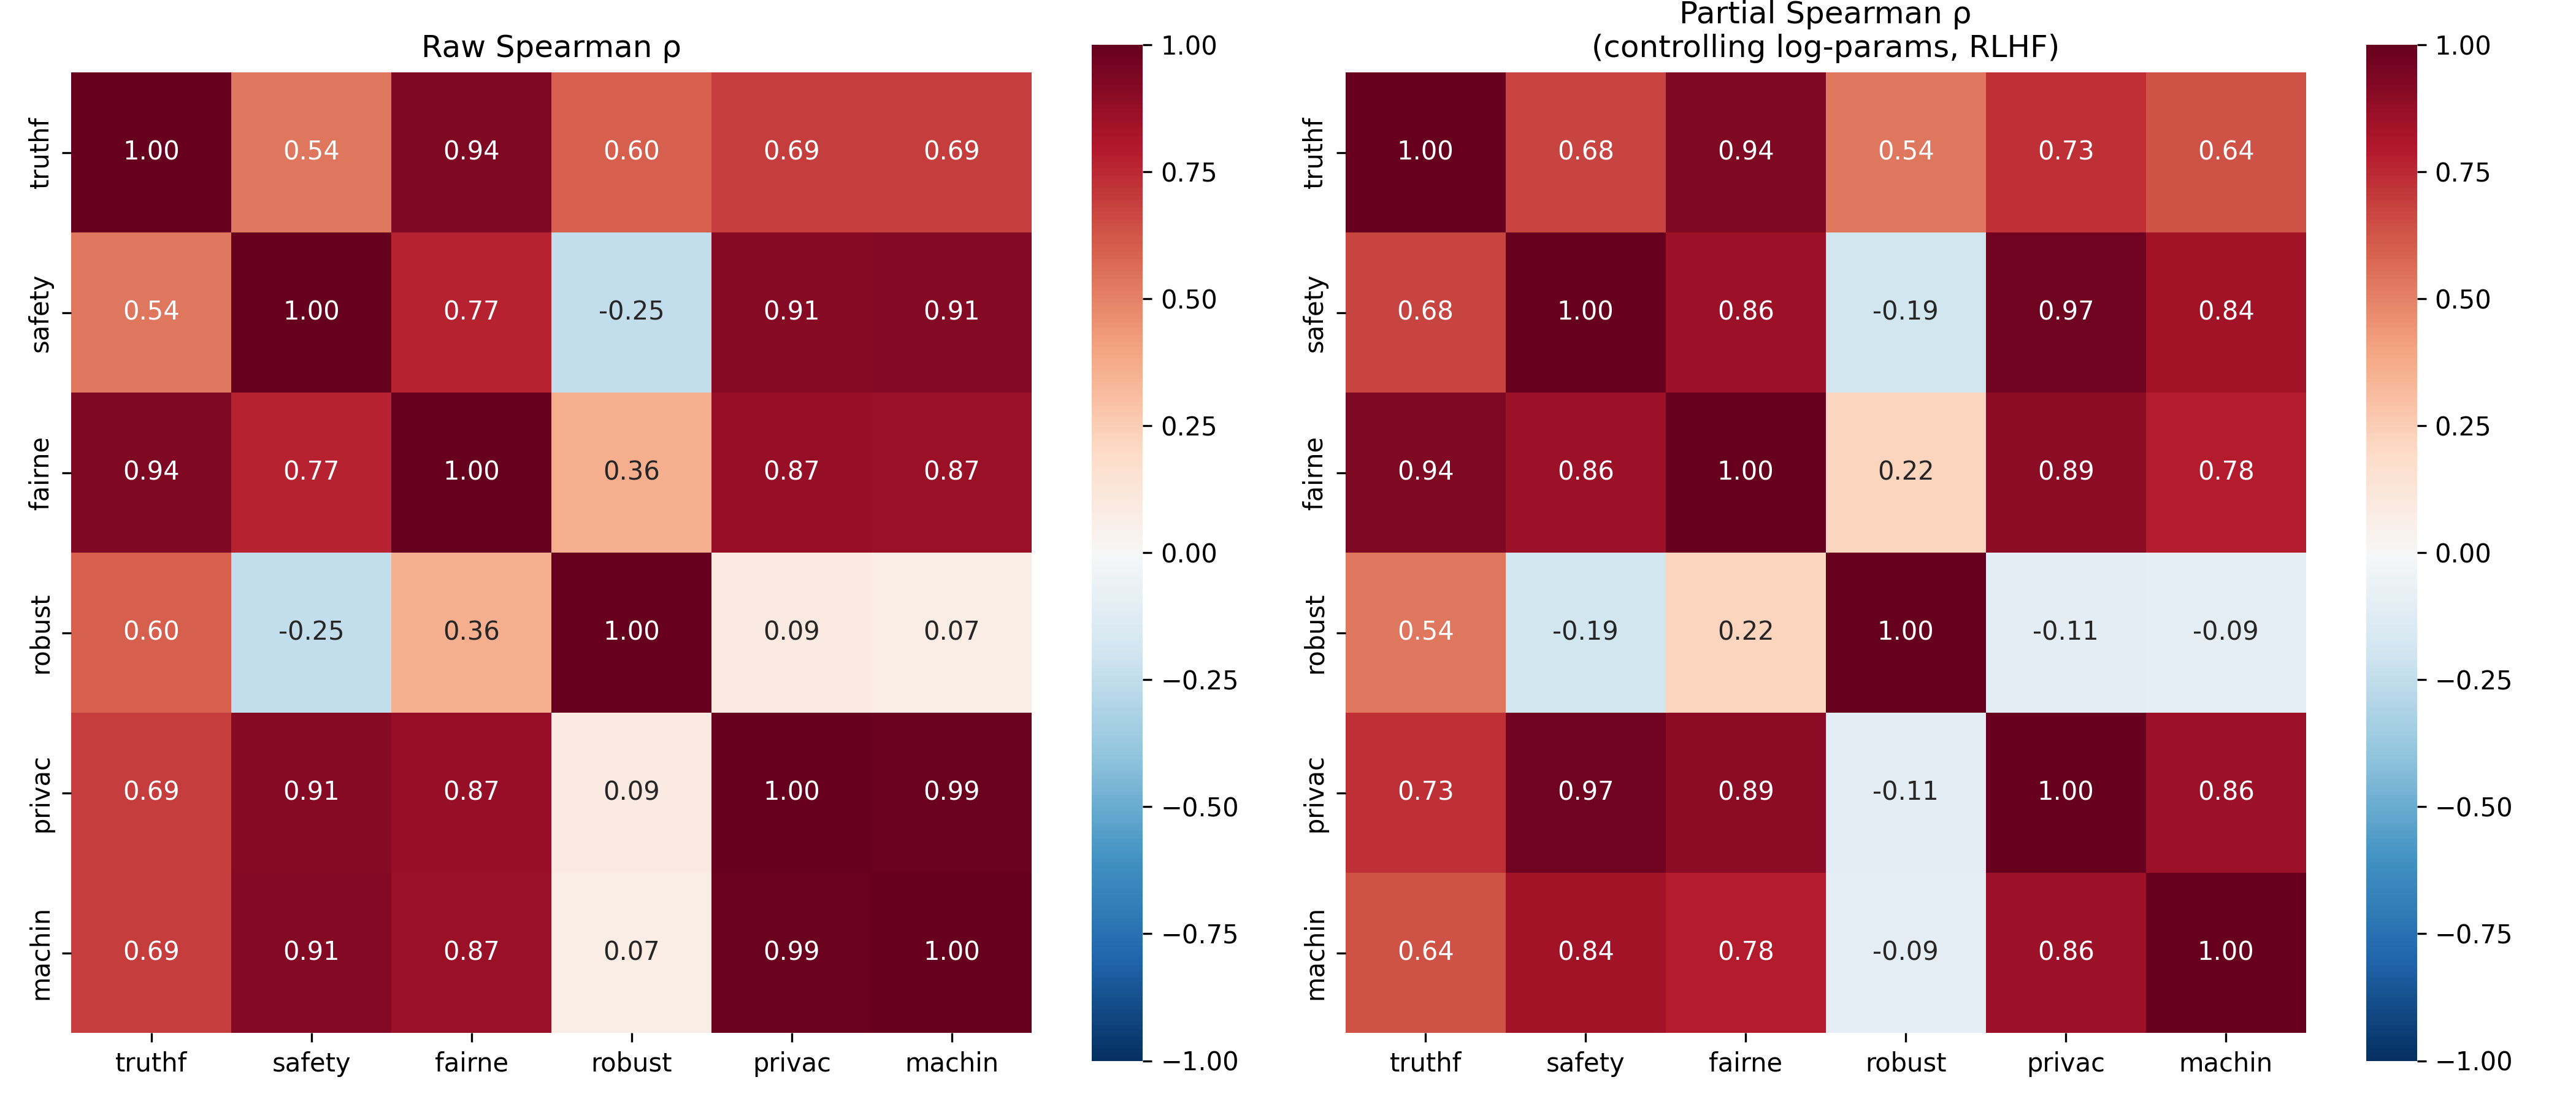
\includegraphics[width=\columnwidth]{figures/02_heatmaps.png}
\caption{Partial vs raw correlation heatmaps}
\label{fig:02_heatmaps}
\end{figure}

\textit{Figure 1: Side-by-side comparison of raw Spearman (left) and partial Spearman (right) $6\times 6$ correlation heatmaps. Controlling for model scale and RLHF status reveals the underlying trustworthiness geometry.}

\begin{figure}[htbp]
\centering
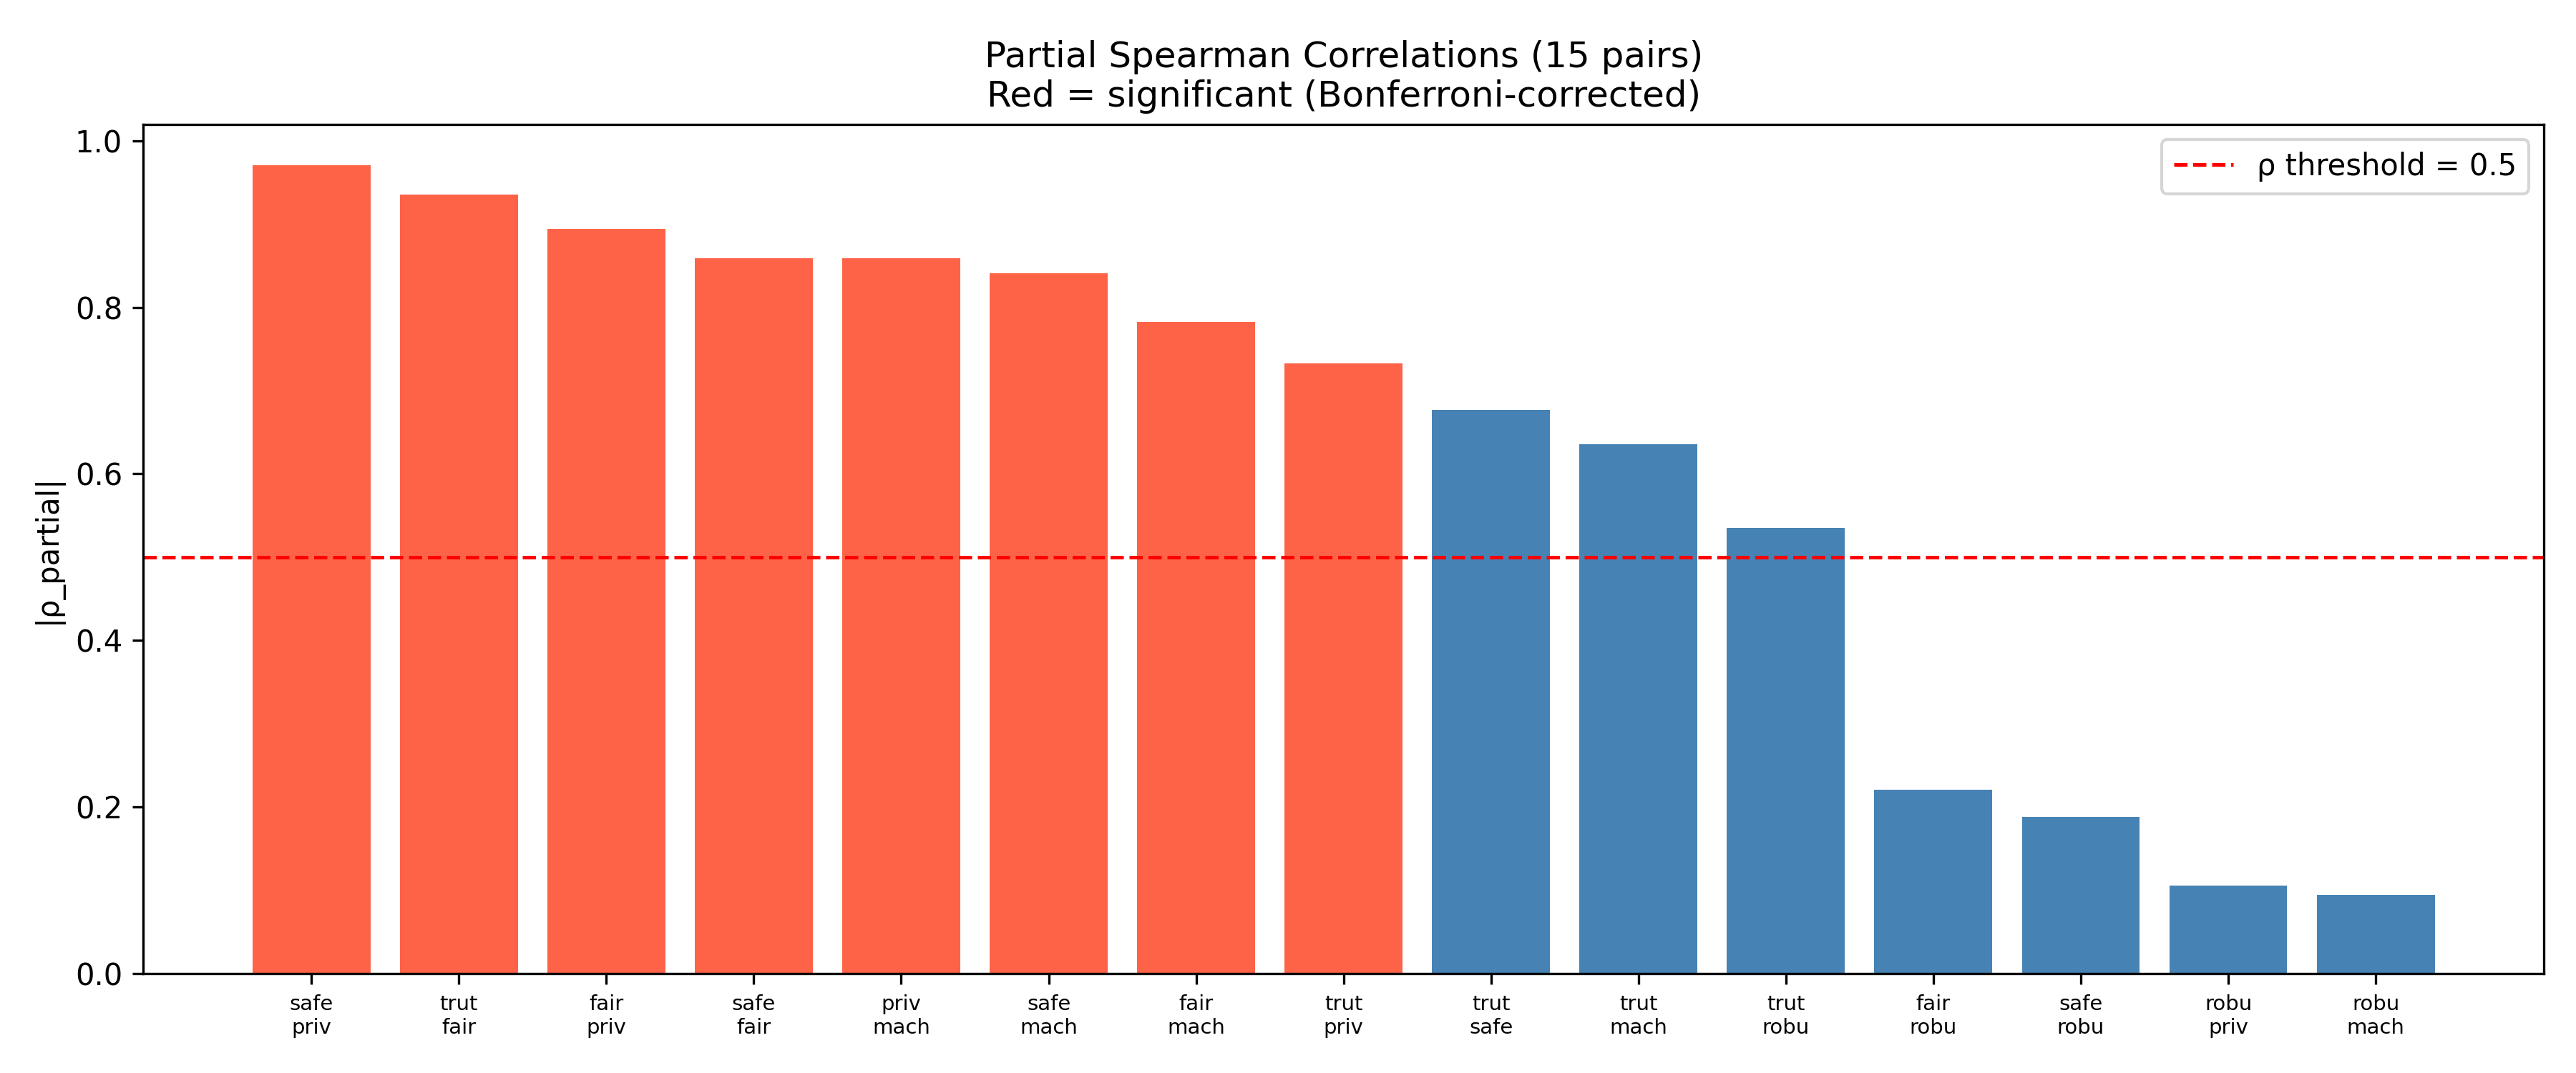
\includegraphics[width=\columnwidth]{figures/01_bar.png}
\caption{Absolute partial correlations bar chart}
\label{fig:01_bar}
\end{figure}

\textit{Figure 2: |$\rho_{partial}$| for all 15 dimension pairs, sorted by magnitude. Red bars indicate Bonferroni-significant pairs (p < 0.0033). 8 of 15 pairs exceed the significance threshold.}

\subsubsection{5.2 RQ2: RLHF Jointly Optimizes Safety and Machine Ethics (H-M1)}

\textbf{Table 2: RLHF-induced deltas in LLaMA-2 within-family pairs}

\begin{table*}[htbp]
\centering
\resizebox{\dimexpr 2\columnwidth+\columnsep\relax}{!}{%
\begin{tabular}{lllll}
\toprule
Scale Pair & $\Delta _safety$ (Chat $-$ Base) & $\Delta _machine_ethics$ (Chat $-$ Base) & $\Delta _robustness$ & Both Safety/Ethics Positive? \\
\midrule
LLaMA-2-7B $\rightarrow$ 7B-Chat & +0.626 & +0.464 & $-0.080$ & Yes \\
LLaMA-2-13B $\rightarrow$ 13B-Chat & +0.652 & +0.422 & $-0.085$ & Yes \\
LLaMA-2-70B $\rightarrow$ 70B-Chat & +0.638 & +0.386 & $-0.094$ & Yes \\
**Mean** & **+0.639** & **+0.424** & **$-0.086$** & **3/3** \\
\bottomrule
\end{tabular}
}
\end{table*}

All 3/3 pairs show joint positive deltas for safety and machine ethics (binomial sign test: p = 0.125, the minimum achievable for n = 3). The directional consistency across three independent scale points provides mechanistic evidence for the joint optimization claim.

For adversarial robustness, all 3/3 pairs show $\Delta _robustness$ < 0. The scale-only control confirms the effect exists: $\rho$(safety, robustness) under scale-only control = $-0.771$ (p = 0.0008). When RLHF status is added as a covariate, this attenuates to $-0.188$ (p = 0.519), suggesting the RLHF binary absorbs shared variance between safety and robustness at the model level.

The partial correlation $\rho_{partial}$(safety, machine\_ethics) = 0.841 (p = 3.22e-05, Bonferroni-significant) confirms that the safety--ethics relationship persists after controlling for both confounders --- it is not merely a reflection of RLHF status.

\begin{figure}[htbp]
\centering
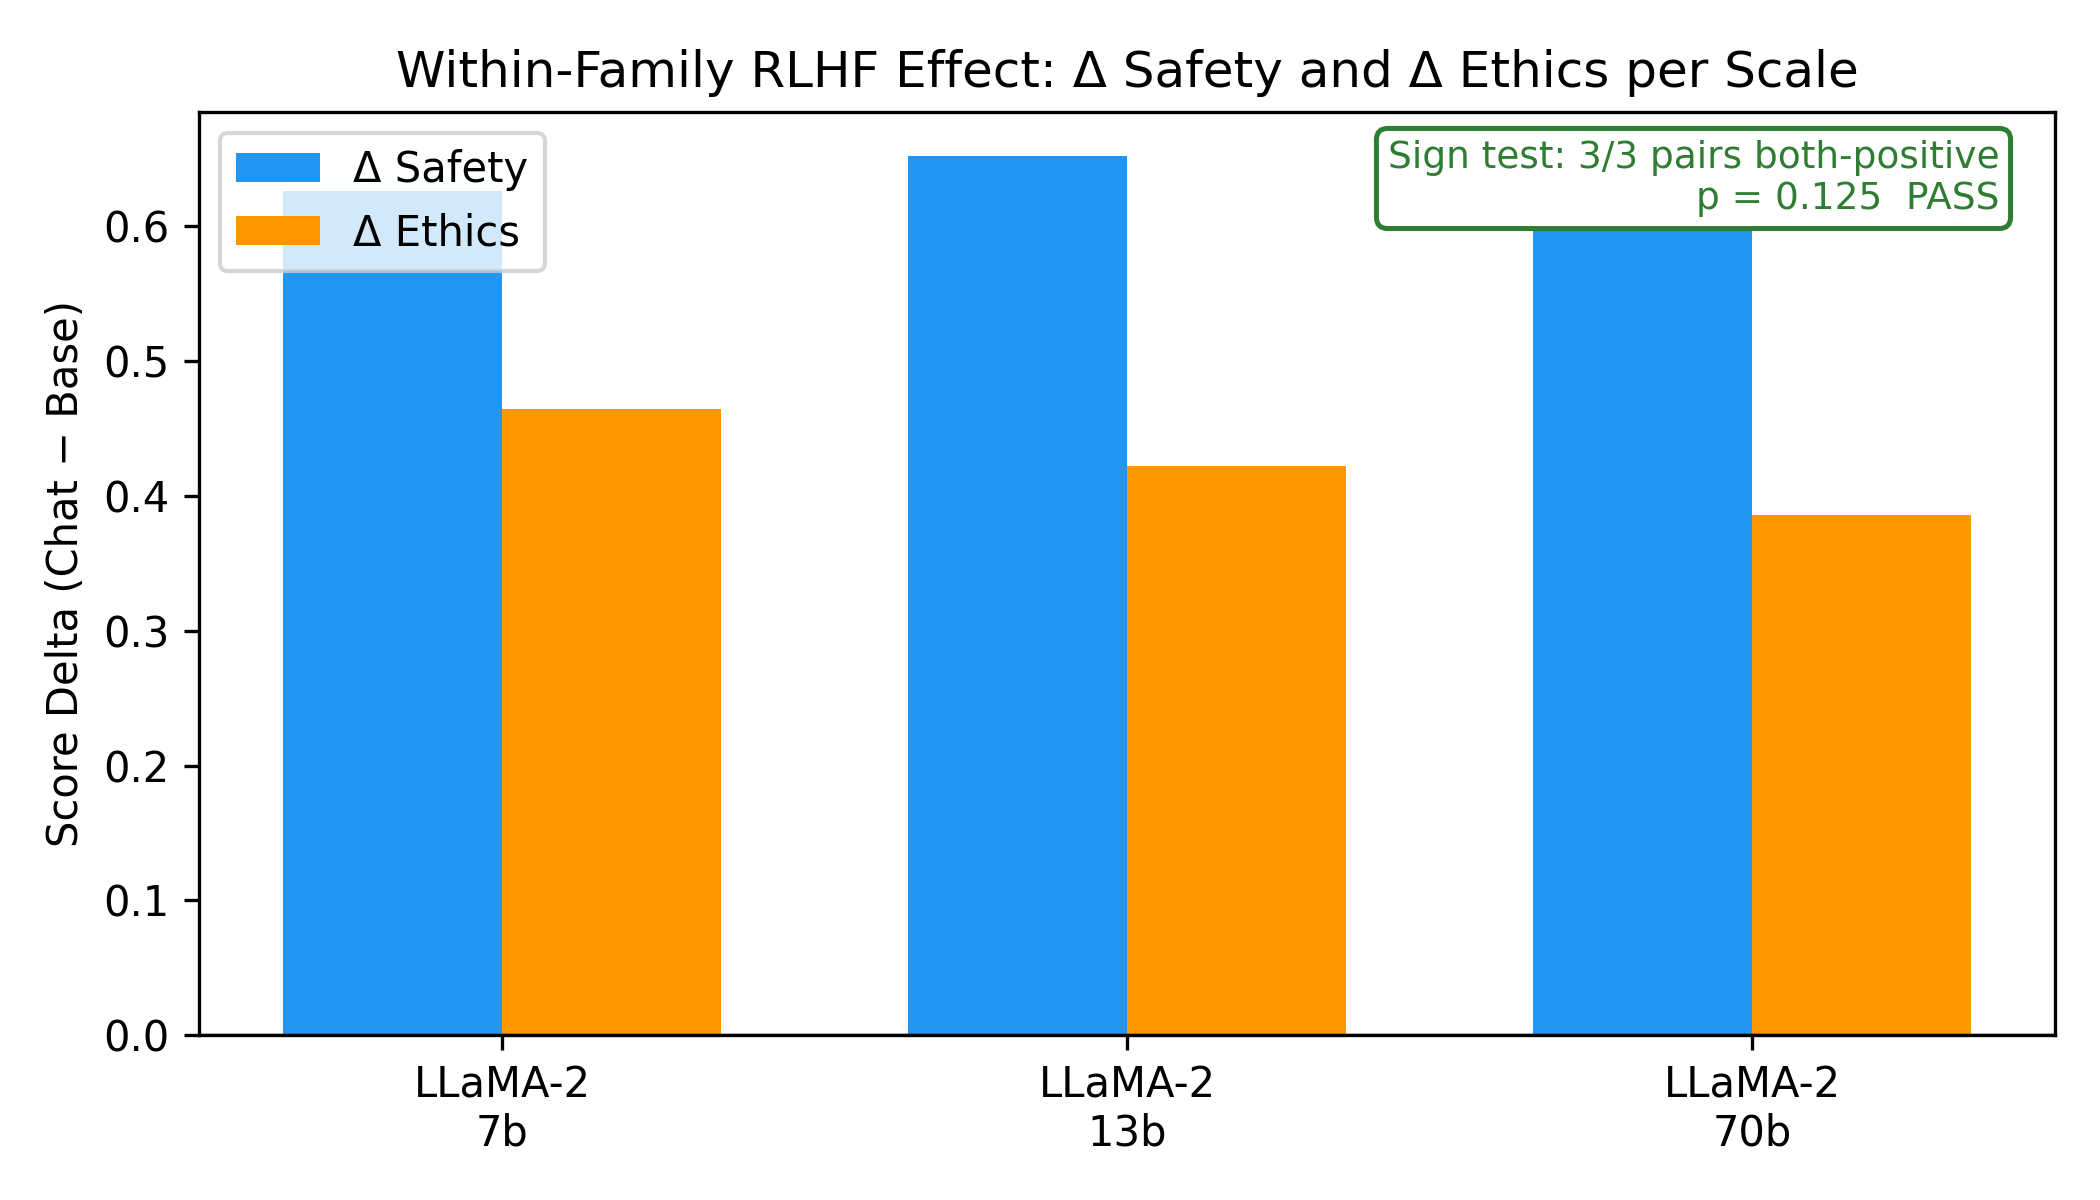
\includegraphics[width=\columnwidth]{figures/fig2_within_family_deltas.png}
\caption{LLaMA-2 within-family RLHF deltas}
\label{fig:fig2_within_family_deltas}
\end{figure}

\textit{Figure 3: RLHF-induced score changes ($\Delta$ = Chat $-$ Base) for safety and machine\_ethics across LLaMA-2 7B, 13B, and 70B. All six bars are positive, demonstrating joint optimization at every scale.}

\begin{figure}[htbp]
\centering
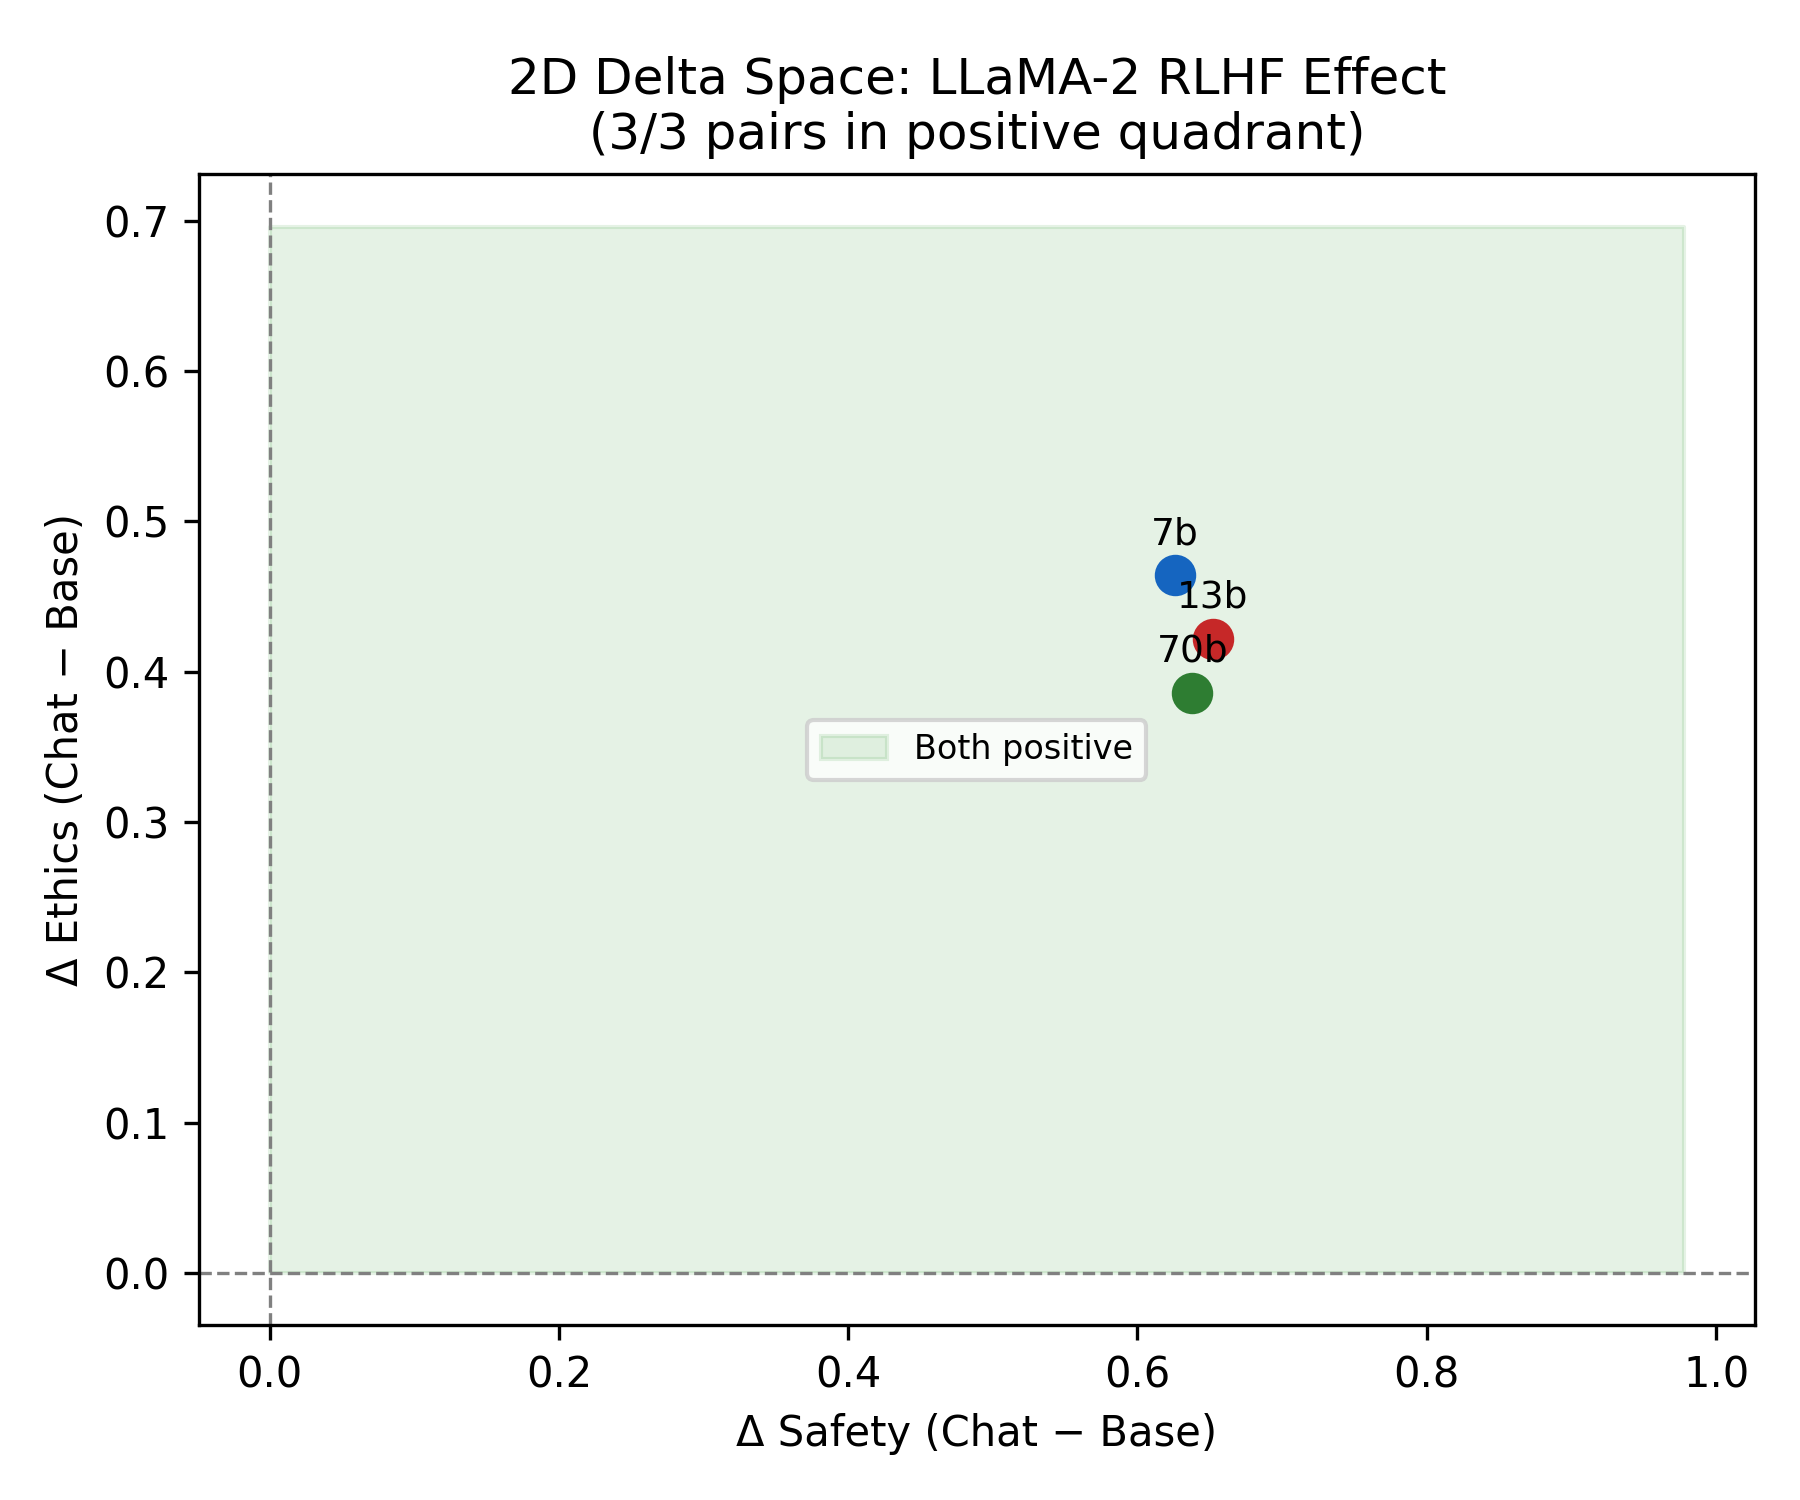
\includegraphics[width=\columnwidth]{figures/fig4_delta_2d.png}
\caption{2D delta space scatter}
\label{fig:fig4_delta_2d}
\end{figure}

\textit{Figure 4: 2D delta space scatter ($\Delta _safety$ vs. $\Delta _machine_ethics)$ for LLaMA-2 within-family pairs. All three scale points land in the upper-right quadrant (both positive).}

\subsubsection{5.3 RQ3: 2-Cluster Structure with Robustness Isolating (H-M3)}

\textbf{Table 3: Silhouette scores by linkage method (distance metric: 1 $- |\rho_{partial}$|)}

\begin{table}[htbp]
\centering
\resizebox{\columnwidth}{!}{%
\begin{tabular}{lll}
\toprule
Linkage & Silhouette (k=2) & Silhouette (k=3) \\
\midrule
Ward & **0.637** & 0.500 \\
Average & **0.637** & 0.500 \\
Complete & **0.637** & 0.500 \\
\bottomrule
\end{tabular}
}
\end{table}

The identical silhouette score of 0.637 across all three linkage methods, and the k=2 substantially outperforming k=3, confirm that the 2-cluster geometry is a genuine data property rather than a methodological artifact of linkage choice.

\textbf{Cluster membership:}
\begin{itemize}
\item \textbf{Cluster A (RLHF-shaped, 5 dimensions):} {truthfulness, safety, fairness, privacy, machine\_ethics}
\item \textbf{Cluster B (RLHF-insensitive, 1 dimension):} {adversarial robustness}
\end{itemize}

The functional split is 1+5. This departs from the original prediction of a 2+4 split ({safety, ethics} vs. {robustness, privacy}). Privacy is in the RLHF-shaped cluster, driven by $\rho$(safety, privacy) = 0.971. The robustness isolation finding is directionally correct.

An alternative distance metric (angular distance: $\sqrt(1 - \rho^{2}))$ produces silhouette = 0.358 (k=2, Ward) --- weaker but still above the 0.3 threshold, providing further geometric confirmation.

\begin{figure}[htbp]
\centering
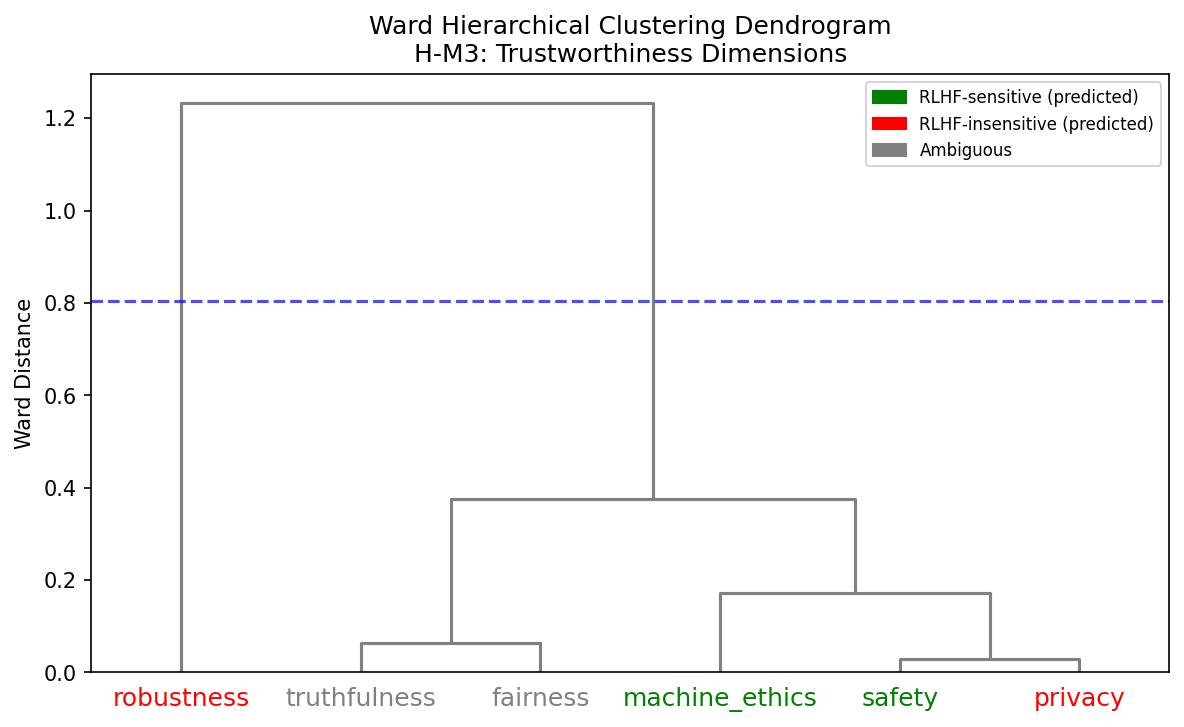
\includegraphics[width=\columnwidth]{figures/dendrogram_ward.png}
\caption{Ward dendrogram}
\label{fig:dendrogram_ward}
\end{figure}

\textit{Figure 5: Ward-linkage dendrogram confirming the 2-cluster structure (silhouette = 0.637). The functional split is {robustness} vs. {all other 5 dimensions}.}

\begin{figure}[htbp]
\centering
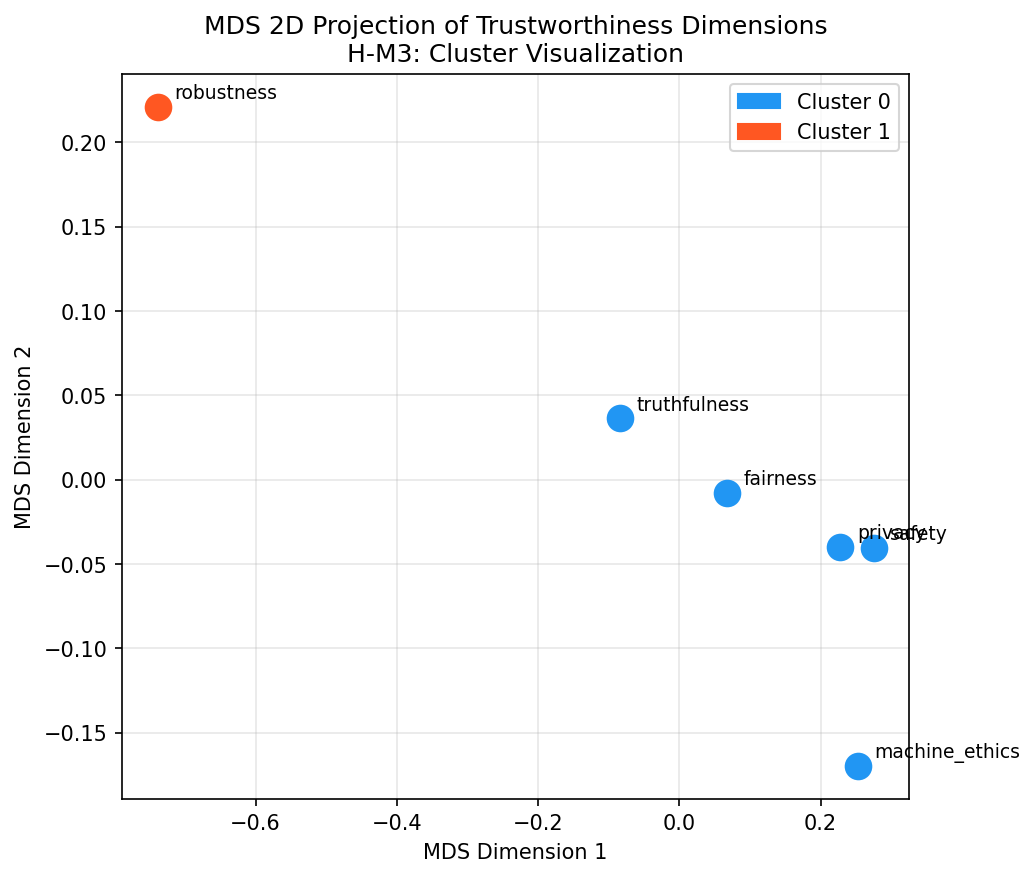
\includegraphics[width=\columnwidth]{figures/mds_projection.png}
\caption{MDS projection}
\label{fig:mds_projection}
\end{figure}

\textit{Figure 6: 2D multidimensional scaling (MDS) projection of the $6\times 6$ partial Spearman distance matrix. Robustness is geometrically separated from the tight 5-dimension cluster.}

\begin{figure}[htbp]
\centering
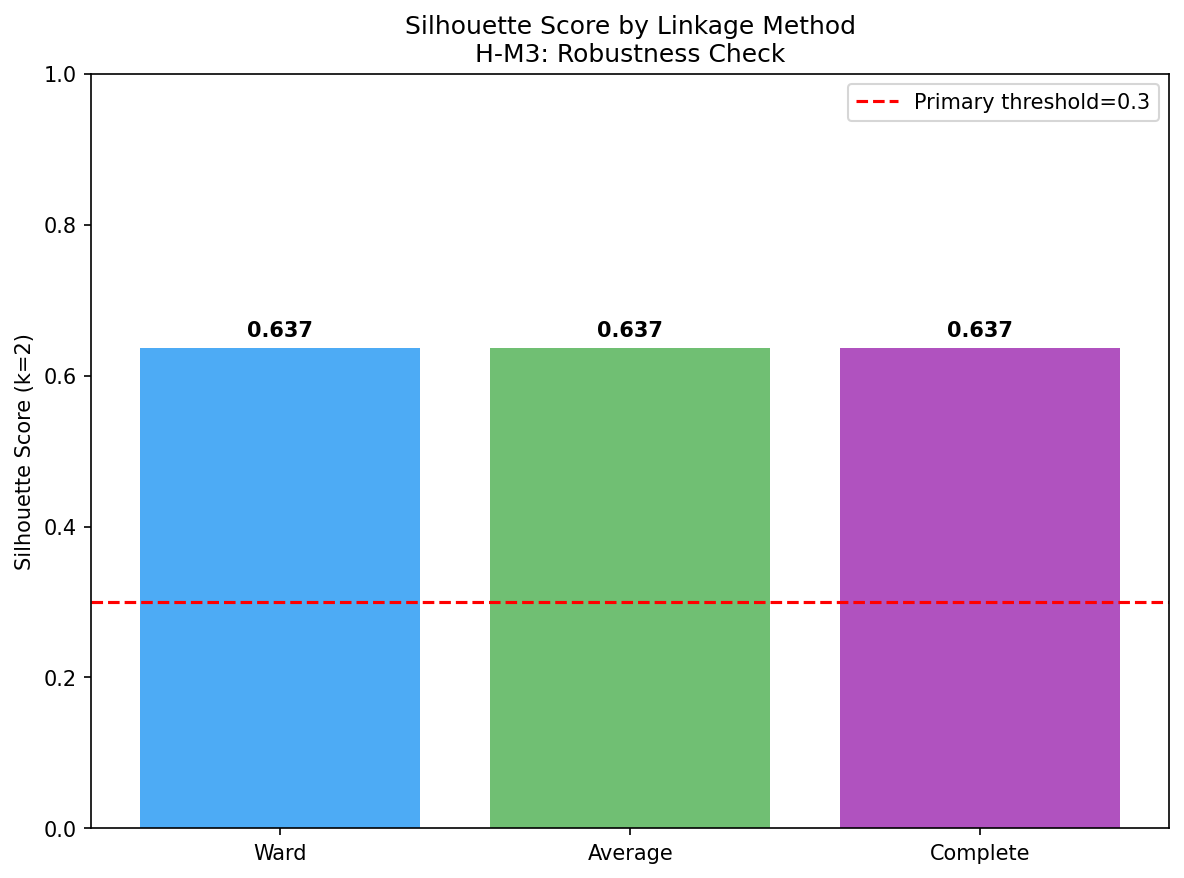
\includegraphics[width=\columnwidth]{figures/silhouette_comparison.png}
\caption{Silhouette comparison}
\label{fig:silhouette_comparison}
\end{figure}

\textit{Figure 7: Silhouette scores for k=2 clustering using Ward, average, and complete linkage methods (all = 0.637) vs. k=3 (0.500). Identical scores across linkage methods confirm the structure is not a methodological artifact.}

\subsubsection{5.4 RQ4: 3-Dimension Minimum Evaluation Set (H-E2-v2)}

\textbf{Table 4: MST edge bootstrap frequencies (1000 resamples of 14/16 models)}

\begin{table*}[htbp]
\centering
\resizebox{\dimexpr 2\columnwidth+\columnsep\relax}{!}{%
\begin{tabular}{lllll}
\toprule
Edge & Distance (1 $-$ & $\rho$ & ) & Bootstrap Frequency \\
\midrule
Privacy --- Safety & 0.029 & 1.000 &  &  \\
Fairness --- Truthfulness & 0.266 & 1.000 &  &  \\
Fairness --- Privacy & 0.088 & 0.956 &  &  \\
Robustness --- Truthfulness & 0.388 & 0.941 &  &  \\
Machine\_Ethics --- Privacy & 0.141 & 0.688 &  &  \\
\bottomrule
\end{tabular}
}
\end{table*}

Mean per-edge bootstrap frequency: \textbf{0.917} (threshold $\geq$ 0.90). The minimum evaluation set {truthfulness, fairness, privacy} is identified from the MST hub nodes (degree > 1).

The machine\_ethics--privacy edge at 68.8\% bootstrap frequency reflects near-tie geometry at n=16: machine\_ethics is approximately equidistant from privacy, safety, and fairness in the 1 $- |\rho$| space (~0.14--0.16). The minimum evaluation set \textit{size} (3 dimensions) is stable; the specific MST attachment of machine\_ethics is ambiguous at this sample size.

\textbf{Comparison with raw (uncontrolled) MST:} The raw Spearman MST requires 4 dimensions to span the correlation space (not 3). Confound removal reduces the minimum evaluation set by one dimension.

\begin{figure}[htbp]
\centering
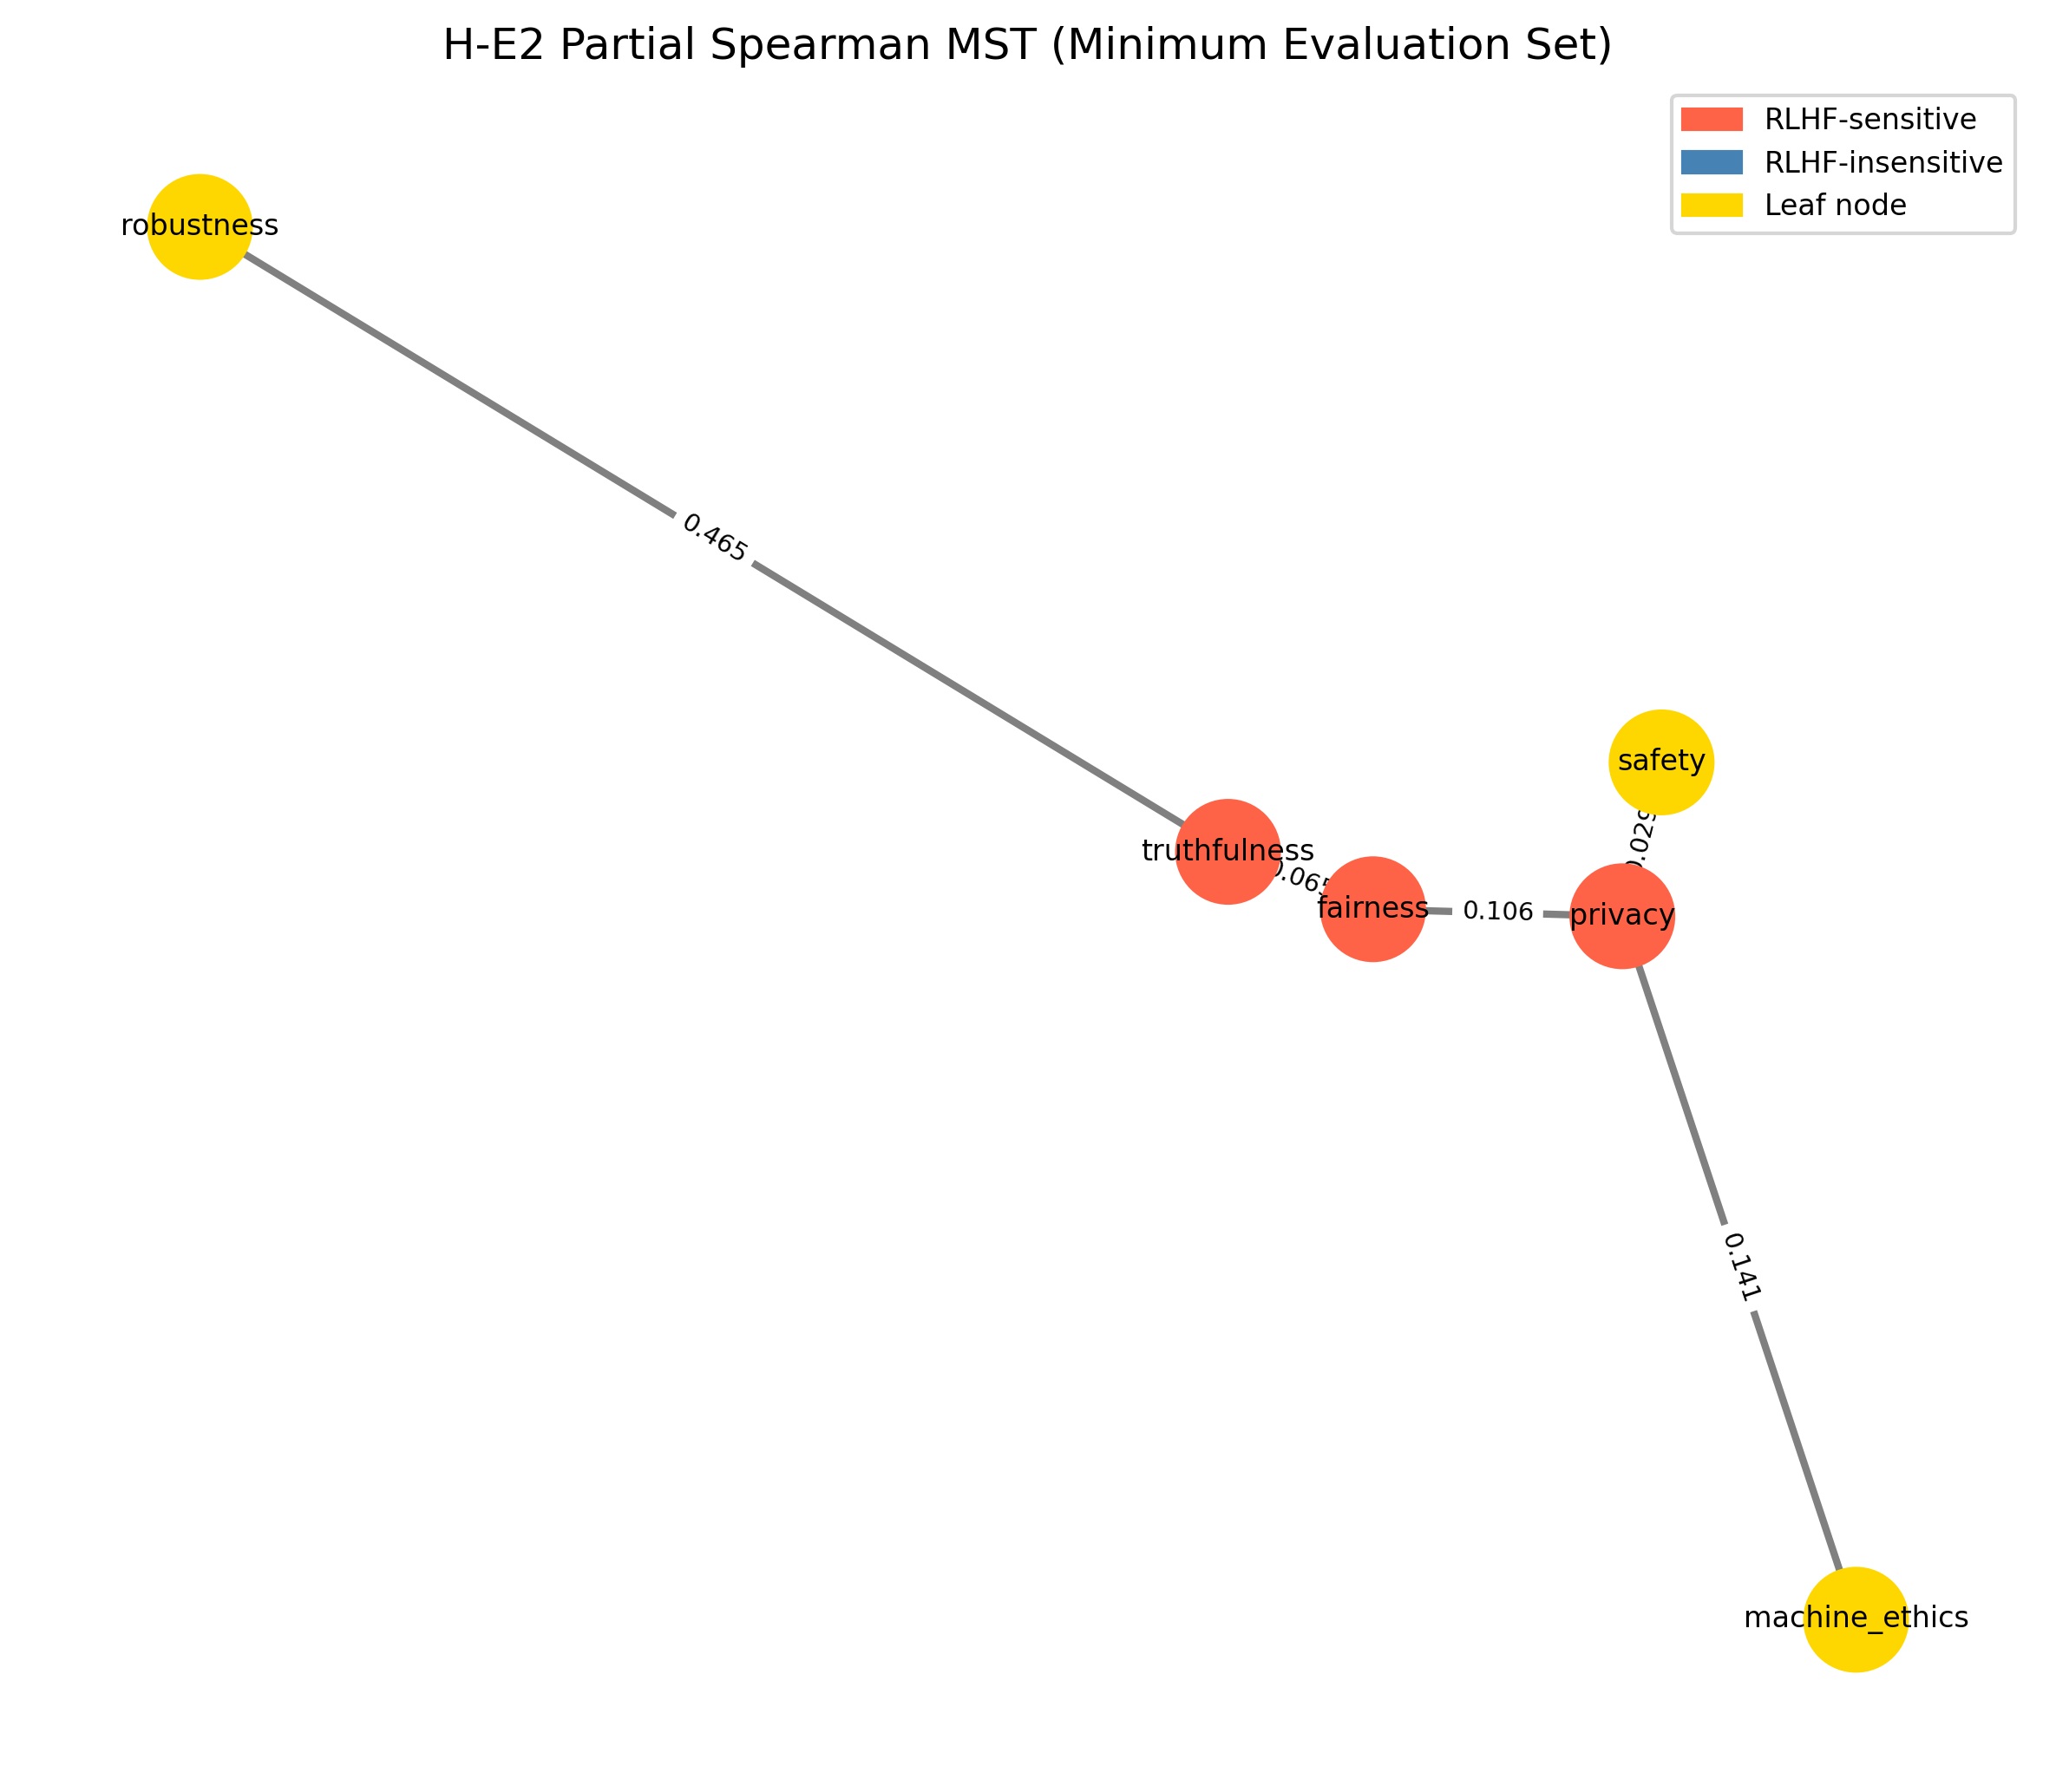
\includegraphics[width=\columnwidth]{figures/mst_graph.png}
\caption{MST graph}
\label{fig:mst_graph}
\end{figure}

\textit{Figure 8: Minimum spanning tree (MST) of the partial Spearman distance matrix. Hub nodes {truthfulness, fairness, privacy} form the 3-dimension minimum evaluation set.}

\begin{figure}[htbp]
\centering
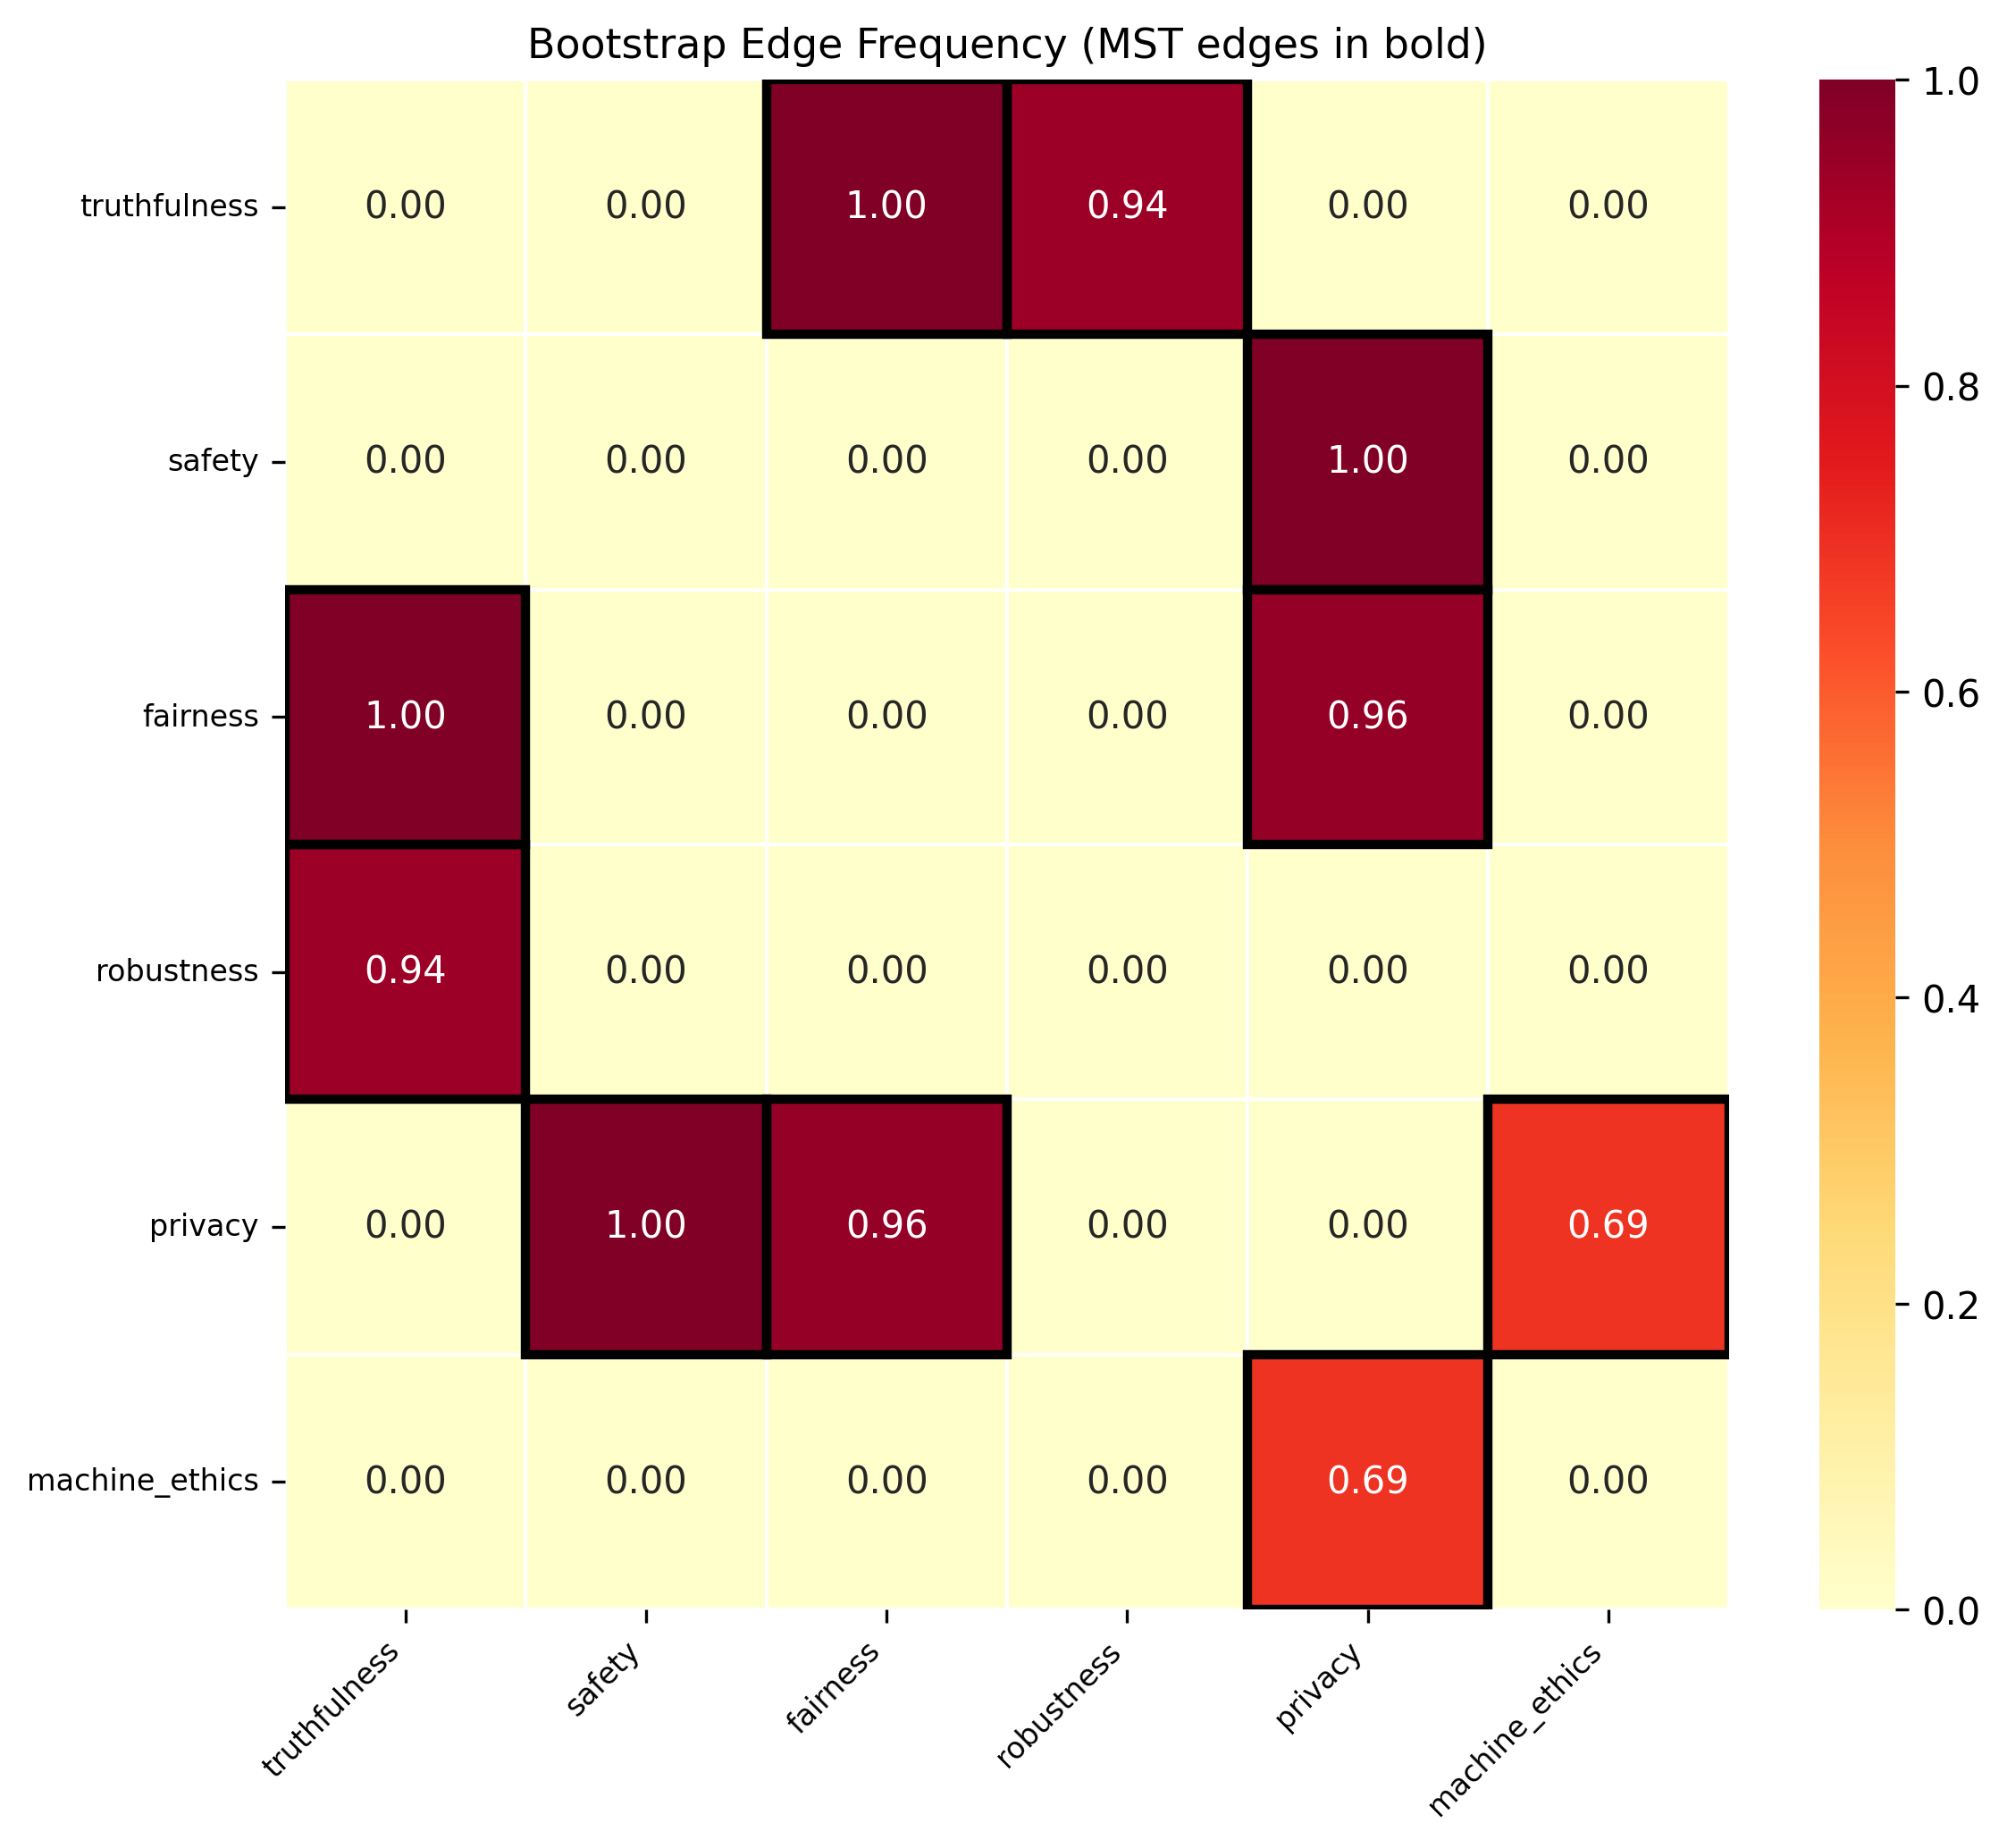
\includegraphics[width=\columnwidth]{figures/bootstrap_heatmap.png}
\caption{Bootstrap frequency heatmap}
\label{fig:bootstrap_heatmap}
\end{figure}

\textit{Figure 9: Per-edge bootstrap frequency heatmap (1000 resamples of 14/16 models). Four of five MST edges exceed 94\% stability. The machine\_ethics--privacy edge at 68.8\% reflects near-tie geometry at n=16.}

